\section{Test af software}
Dette afsnit beskriver, hvordan softwaren er testet, samt hvordan dette er dokumenteret. Som udgangspunkt er ideen med softwaretest altid at lave unittest, integrationstest og til sidst systemtest. Som nævnt ganske kort i afsnittet software design, så viste det sig at være sværere at unitteste softwaren end forventet. Dette tyder på at selvom softwaren er designet ud fra ideen om lav kobling, så har dette ikke været opfyldt tilstrækkeligt. 
Følgende elementer er blevet unittestet: Pulsalgoritmen, blodtryksalgoritmen, det digitale filter og lineær regressionsberegning i forbindelse med kalibrering. Se dokumentet Softwaretest for dokumentation af disse tests. 
En af de udførte unittests er som nævnt test af det digitale filter. Dette blev gjort ved at lave et sinussignal med hvid støj, som blev sendt igennem filteret. Nedenstående figur viser sammenligning mellem det filtrede og ufiltrerede signal. 

\vspace{0.5 cm}
\begin{figure}[h!]
	\centering
	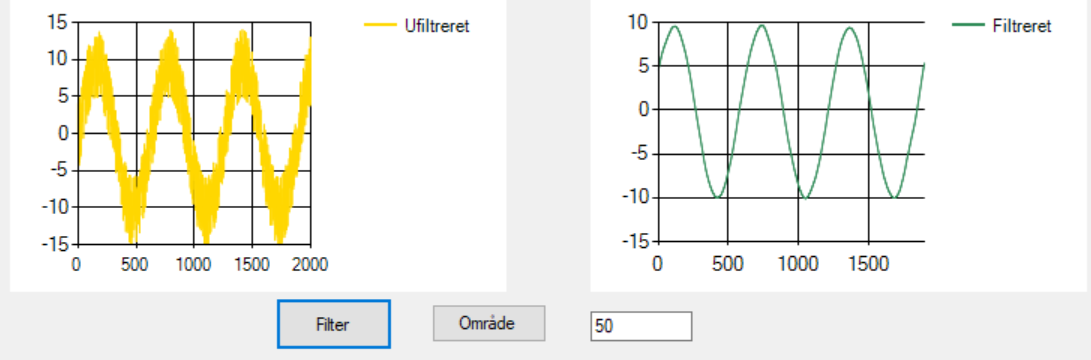
\includegraphics[width=1\linewidth]{Implementering_og_test/Software/filter_test}	
	\caption{Test af det digitale filter}
	\label{fig:ufiltreret}
\end{figure}

Som nævnt i indledningen var det meget svært at lave unittest på vores use cases. Det endte derfor med at langt det meste softwaretest har været integrationstest, hvor hele use casen er testet på én gang. Dette blev gjort ved hjælp af debuggeren i Visual Studio. Ved at sætte breakpoints i koden og følge de forskellige kald ned gennem koden kunne fejl lokaliseres på denne måde. Problemet ved at bruge debuggeren og ikke skrive en selvstændig testsuite er en mangelfuld dokumentation af disse tests. Dette giver sig til udtryk i softwaretest (eller hvad det hedder) dokumentet, som kun indeholder de beskrevne unittests og ikke integrationstest. Dette kom også til udtryk under udførelsen af accepttest, hvor flere tests ikke opførte sig som forventet, hvilket igen indikerer en utilstrækkelig systematisk tilgang til test. 

\textbf{Systemtest}

To andre væsentlige tests, som ikke kom med i vores accepttest, er test af nøjagtighed og præcision af vores system. Præcision af vores system vil vi teste ved at lave en måling på et minut, det vil sige 60.000 samples, ved et tryk på 100 mmHg og derefter beregne standardafvigelsen på målingerne. 

Nøjagtighed vil vi teste ved at kalibrere flere gange og derefter måle et kendt tryk. Ud fra dette kan vi konkludere på, hvor meget vores system afviger fra det kendte signal. Her skal det dog nævnes, at denne test er vanskelig på grund af kalibreringen, som bliver lavet ved hjælp af væskesøjlen, hvor det kendte tryk manuelt skal indstilles ved at hælde vand i søjlen. Dette betyder, at det kendte signal i realiteten ikke er 100 \% kendt og kalibreringen vil derfor afvige en smule fra gang til gang. En ordentlig test af nøjagtig vil derfor kræve andet udstyr til kalibrering. 

